\documentclass{tufte-handout}
\usepackage[utf8]{inputenc}
\usepackage{parskip}
\usepackage{amssymb, amsthm, amsmath, fdsymbol, mathtools, cancel, extarrows} % Varios paquetes para símbolos y fuentes
\usepackage{tikz, pgfplots} % Para dibujar
\usepackage{tkz-graph, tkz-berge} % Para dibujar grafos
\usepackage[linguistics]{forest} % Para dibujar árboles
\useforestlibrary{edges}
\usepackage{algorithm2e} % Para escribir pseudocódigo
\usepackage{titling} % Para estilizar el título
\usepackage{scrextend} % Añade márgenes para hacer bloques de texto
\usepackage{enumitem} % Para enumerar sin sangría
\usepackage{graphicx, subcaption} % Para colocar figuras e imágenes
\usepackage{lastpage}
\usepackage{fancyhdr} % Para hacer encabezados y pie de página más estilizados
\usepackage{color} % Para usar colores en el texto
\usepackage{soul} % Para subrayar con colores
\usepackage{soulutf8}
\usepackage{titling} % Cambia los parámetros del título
\usepackage{booktabs} % Para hacer tablas un poco más estilizadas
\usepackage{multirow}
\usepackage[font={footnotesize}]{caption} % Cambia el tamaño de los captions
\usepackage{subcaption} % Para referenciar subfiguras
\usepackage{hyperref}

% Establece el subrayado de color rojo
\definecolor{ferrari}{rgb}{1,0.17,0}
\setulcolor{ferrari}

% Agrega etiquetas con colores a las matrices
\usepackage{colortbl}
\usepackage{nicematrix}
\NiceMatrixOptions{
code-for-first-row = \color{red} ,
code-for-last-row = \color{red} ,
code-for-first-col = \color{red} ,
code-for-last-col = \color{red}
}

\tikzset{unode/.style = {
    circle, 
    draw=black, 
    thick,
    fill=black,
    inner sep=2.3pt,
    minimum size=2.3pt } }
\tikzset{uedge/.style = {
    draw=black, 
    very thick} }

% Establece los enviroments para teoremas, ejemplos, definiciones, etc
\newtheorem{teo}{Teorema}
\newtheorem{cor}[teo]{Corolario}
\newtheorem{lem}[teo]{Lema}
\newtheorem{pro}[teo]{Proposición}
\newtheorem{pre}{Pregunta}

\theoremstyle{definition}
\newtheorem{defn}{Definición}
\newtheorem{ejem}{Ejemplo}
\newtheorem{ejer}{Ejercicio}
\newtheorem{notn}{Notación}
\newtheorem{nota}{Nota}
\newtheorem{prob}{Problema}

% Comandos para símbolos
\newcommand{\Nastk}{\mathbb{N}^*}
\newcommand{\N}{\mathbb{N}}
\newcommand{\Z}{\mathbb{Z}}
\newcommand{\R}{\mathbb{R}}
\newcommand{\lngtd}[1]{\operatorname{long}(#1)}
\newcommand{\LC}{\nameref{teo:primer}}

% Cambia el nombre de varios comandos
\renewcommand{\contentsname}{Contenido}
\renewcommand*{\proofname}{Demostración}
\renewcommand{\figurename}{Fig.}

% Resetea el contador de ecuaciones en cada sección y/o subsección
\newcounter{sec}
\newcounter{subsec}
\setcounter{sec}{0}
\setcounter{subsec}{0}
\counterwithin*{equation}{sec}
\counterwithin*{equation}{subsec}

% Establece las notas de margen
\newcommand{\marginfootnote}[1]{\footnotemark\footnotetext{#1}}

% Establecemos cómo será el encabezado y el pie de página
\fancyhf{}
\pagestyle{fancy}
\fancyhf{}
\fancyhead[L]{MA-5274}
\fancyhead[C]{Eduardo José Gavazut Pinto}
\fancyhead[R]{13-10524}
\fancyfoot[L]{Sección 1}
\fancyfoot[R]{Profesor: Jesús Nieto}
\fancyfoot[C]{\thepage\ de \pageref{LastPage}}
\renewcommand{\headrulewidth}{2pt} 
\renewcommand{\footrulewidth}{2pt}

% Establece los entornos para los bloques de pseudocódigo
\RestyleAlgo{ruled}
\newenvironment{algoritmo}[1][htb]
  {\renewcommand{\algorithmcfname}{Algoritmo}% Update algorithm name
   \begin{algorithm}[#1]%
  }{\end{algorithm}}

\newcommand{\row}[1]{%
  \hbox{$\activatem\romannumeral\number\number#1 000 \unskip$}\vskip 0.5em plus 3em
}
\newcommand{\activatem}{%
  \begingroup\lccode`~=`m \lowercase{\endgroup\def~}{\bullet\hskip1em}%
  \mathcode`m="8000
}

% Define la geometría del margen
\geometry{
	left=13mm, % left margin
	textwidth=130mm, % main text block
	marginparsep=8mm, % gutter between main text block and margin notes
	marginparwidth=55mm % width of margin notes
}

% Permite agregar etiquetas a los niveles de un árbol
\forestset{%
  label tree/.style={
    for tree={tier/.option=level},
    level label/.style={
      before typesetting nodes={
        for nodewalk={current,tempcounta/.option=level,group={root,tree breadth-first},ancestors}{if={>OR={level}{tempcounta}}{before drawing tree={label me=##1}}{}},
      }
    },
    before drawing tree={
      tikz+={\coordinate (a) at (current bounding box.east);},
    },
  },
  label me/.style={tikz+={\node [anchor=base north] at (.parent |- a) {#1};}},
}

% Reduce el espacio entre el título y el header
\setlength{\droptitle}{-5.5em}
\renewcommand\maketitlehookc{\vspace{-3ex}}

% Define el espaciado entre párrafos
\setlength{\parskip}{1.5em}

% Definimos nuestro título
\pretitle{\begin{flushleft}\LARGE\sffamily}
\title{
Notas de Teoría de Grafos I, Septiembre-Diciembre 2022 \\
Universidad Simón Bolívar
}
\posttitle{\par\end{flushleft}\vskip 0.5em}
\preauthor{\begin{flushleft}\large\scshape}
\author{
Eduardo Gavazut \\
Carnet: 13-10524}
\postauthor{\par\end{flushleft}}
\predate{\begin{flushleft}\large\scshape}
\date{Septiembre-Diciembre 2022}
\postdate{\par\end{flushleft}}

% Aquí empieza el documento
\begin{document}

\maketitle
\thispagestyle{fancy}

\tableofcontents
\break
\section{Conceptos Fundamentales}

Este curso sigue los tres primeros capítulos de Introduction to Graph Theory de West. Esto comprende grafos, conteo, árboles, matching, teoremas de cubrimiento y una introducción a la factorización de grafos. Por lo tanto, es fundamental estudiar con el libro a la hora de revisar este curso y buscar ejercicios.

\subsection{Definiciones básicas}

\begin{defn}
    Un \ul{grafo} es una tripleta $G = (V(G, E(G), f_G)$ en el cual $V(G)$ y $E(G)$ son conjuntos y $f_G$ es una función que asigna a cada $e \in E(G)$ un \textbf{par no ordenado} $\{x,y\} \subset V(G)$.
\end{defn}

\begin{prob}[El problema de los puentes de Könisberg]\label{prob:konisberg}

    \begin{marginfigure}
        \centering
        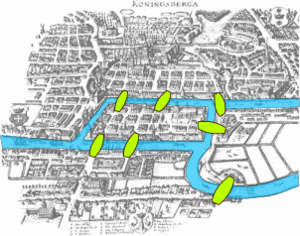
\includegraphics[scale=0.5]{img/konisberg.png}
        \caption{Parte del mapa de la ciudad de Könisberg. En verde están reflejados los puentes descritos en el problema.}
        \label{fig:konisberg}
    \end{marginfigure}
    
    La ciudad de Könisberg se encontraba ubicada sobre el río Pregel en Prusia. La ciudad ocupaba dos islas más dos áreas sobre ambas orillas. Estas regiones se encontraban unidas por $7$ puentes. La gente en la ciudad empezó a preguntarse si podían salir de sus hogares, cruzar cada puente exactamente una vez y regresar a casa.
    
    \begin{marginfigure}
        \centering
        \begin{tikzpicture}
            \SetGraphUnit{2}
            \Vertices{circle}{d,c,b,a}
            \Edge[label=$e_6$](c)(d)
            \Edge[label=$e_7$](c)(b)
            \Edge[label=$e_3$](a)(c)
            \tikzset{EdgeStyle/.append style = {bend left}}
            \Edge[label=$e_1$](a)(b)
            \Edge[label=$e_2$](b)(a)
            \Edge[label=$e_4$](a)(d)
            \Edge[label=$e_5$](d)(a)
        \end{tikzpicture}
        \caption{Grafo que representa la situación descrita en el problema \ref{prob:konisberg}.}
        \label{fig:konisberg-model}
    \end{marginfigure}
    
    Este problema puede ser analizado a través de un grafo: Etiquetamos las $4$ regiones de la figura \ref{fig:konisberg} y graficamos como en la figura \ref{fig:konisberg-model}. Vemos que en este caso,
    
    \begin{itemize}
        \item $V(G) = \{a, b, c, d\}$.
        \item $E(G) = \{e_1, e_2, e_3, e_4, e_5, e_6, e_7\}$.
        \item $f_G(e_1) = \{a,b\} = f_g(e_2)$, $f_G(e_3) = \{a,c\}$, $f_G(e_4) = \{a,d\} = f_G(e_5)$, $f_G(e_6) = \{d,c\}$ y $f_G(e_7) = \{b,c\}$.
    \end{itemize}
    
    Más adelante responderemos la pregunta que plantea el problema. Por ahora nos limitaremos a revisar más definiciones.
\end{prob}

\begin{defn}[Vocabulario]
    A los elementos de $v \in V(G)$ les llamaremos \ul{vértices} y a los de $e \in E(G)$ les llamaremos \ul{lados o arista}. Dados $v, w \in V(G)$ tales que $\{v, w\} = f_G(e)$ para algún $e \in E(G)$, entonces $v$ y $w$ son \ul{vecinos o adyacentes}.
    
    En un grafo es posible que un vértice sea vecino de sí mismo, y en este caso decimos que el lado correspondiente es un \ul{bucle}.
    
    \begin{marginfigure}
        \centering
        \begin{tikzpicture}
            \SetGraphUnit{2}
            \Vertex{a}
            \EA(a){b}
            \Edge(a)(b)
            \Loop[dist=2cm](a)
        \end{tikzpicture}
        \caption{Ejemplo de un grafo con bucle en el vértice $a$.}
    \end{marginfigure}
    
    Decimos que el grafo $G$ es \ul{simple} si no tiene bucles y $f_G$ es inyectiva (es decir que no tiene lados paralelos como en el grafo de la figura \ref{fig:konisberg-model}). En este caso se identifica a $E(G)$ con el rango de $f_G$. Es decir, los lados son los pares no ordenados de vértices adyacentes.
\end{defn}

\begin{defn}
    Un \ul{clique} en un grafo es un conjunto de vértices que tienen la propiedad de que todos los vértices son vecinos entre sí. En general, un clique es un conjunto de vértices que son adyacentes dos a dos.
    
    Un conjunto de vértices es \ul{independiente} si sus elementos son no adyacentes dos a dos.
\end{defn}

\begin{prob}\label{prob:2}
    En todo grupo de seis personas, hay tres que se conocen o tres que son mutuamente desconocidos. Es decir, ¿es cierto que en todo grafo con $6$ vértices hay un clique con tres vértices o un conjunto independiente con tres vértices?
    
    \begin{marginfigure}
        \centering
        \begin{tikzpicture}
            \GraphInit[vstyle=Normal]
            \SetVertexNoLabel
            \grComplete[RA=2]{6}
            \end{tikzpicture}
        \caption{Cada vértice representa a una persona.}
        \label{fig:3conocidos}
    \end{marginfigure}
    
    Para analizar este problema, etiquetamos a las personas del grupo y las emparejamos como en la figura \ref{fig:3conocidos}. Vemos que para todo vértice $i$, $\{i,j\} \in E(G)$ para todo $j \neq i$. Ahora procedamos a pintar los lados del grafo de la siguiente manera: Para todo lado $\{i,j\}$, si $i$ conoce a $j$ lo pintamos de rojo, de lo contrario se elimina el lado.
    
    \begin{marginfigure}
        \centering
        \begin{tikzpicture}
            \GraphInit[vstyle=Normal]
            \SetGraphUnit{2}
            \Vertices{circle}{$v$,$v_1$,$v_2$,$v_3$,$v_4$,$v_5$}
            \tikzset{
                EdgeStyle/.append style = {red}
            }
            \Edges[color=red]($v$,$v_1$,$v$,$v_2$,$v$,$v_3$)
        \end{tikzpicture}
        \caption{Pintamos los lados de color rojo como lo describimos en el problema.}
        \label{fig:3conocidos-rojo}
    \end{marginfigure}
    
    Entonces, fijémonos en un vértice $v$. Para el resto de los $5$ vértices, cada lado correspondiente lo podemos pintar de rojo o no son adyacentes, y por el principio del casillero, hay al menos $3$ lados pintados de un solo color o que no son adyacentes. Supongamos que están pintados de rojo, y llamemos a los vértices $v_1$, $v_2$, $v_3$ como en la figura \ref{fig:3conocidos-rojo}. Si alguno de los lados $\{v_1, v_2\}$, $\{v_2, v_3\}$ ó $\{v_1, v_3\}$ está pintado de rojo, entonces tenemos un clique de tres vértices donde cada lado es de color rojo. Por el contrario, si los tres lados no son adyacentes entre sí, entonces tenemos un conjunto independiente.
    
    De cualquier manera, tenemos $3$ personas que se conocen (clique rojo) o tres personas que no se conocen (conjunto independientes).
\end{prob}

Las definiciones de clique y complemento dan pie a la definición de complemento de un grafo:

\begin{defn}
    El \ul{complemento} de un grafo simple $G$ es el grafo simple $\overline{G}$ tal que $V(\overline{G}) = V(G)$ y $e \in E(\overline{G})$ sii $e \notin E(G)$. En este sentido, $V(G)$ es un clique si y sólo si $V(\overline{G})$ es un conjunto independiente
\end{defn}

\begin{defn}
    El grafo $G$ es \ul{bipartito} si $V(G)$ es unión de dos conjuntos independientes disjuntos. En general, si $V(G)$ es unión de $k$ conjuntos independientes entonces decimos que $G$ es $k$-partito.
\end{defn}

\begin{prob}
    Tenemos $m$ trabajos que queremos asignar a $n$ personas, pero no todas las personas están calificadas para todos los trabajos. ¿Podemos llenar las vacantes con personas calificadas?
    
    Este problema puede modelarse con un grafo $H$ donde cada vértice representa una persona ó un trabajo. El trabajo $t$ es adyacente a la persona $p$ si $p$ puede hacer $j$. Cada trabajo es realizado por exactamente una persona, por lo tanto estamos buscando $m$ lados disjuntos dos a dos. Un ejemplo de esto puede verse en la figura \ref{fig:trabajos-personas}.
    
    \begin{marginfigure}\label{fig:trabajos-personas}
        \centering
        \begin{tikzpicture}
            \GraphInit[vstyle=Welsh]
            \Vertex{a}
            \Vertex[x=1 , y=0]{b}
            \Vertex[x=2 , y=0]{c}
            \Vertex[x=3 , y=0]{d}
            \Vertex[x=0 , y=2]{1}
            \Vertex[x=1 , y=2]{2}
            \Vertex[x=2 , y=2]{3}
            \Vertex[x=3 , y=2]{4}
            \Edge(1)(a)
            \Edge(1)(b)
            \Edge(1)(c)
            \Edge(1)(d)
            \Edge(2)(a)
            \Edge(2)(d)
            \Edge(3)(b)
            \Edge(3)(c)
            \Edge(4)(a)
            \Edge(4)(c)
            \Edge(4)(d)
            \AddVertexColor{red}{1,2,3,4}
            \AddVertexColor{blue}{a,b,c,d}
            \node[xshift=-1.2cm] at (0,2) {personas};
            \node[xshift=-1.2cm] at (0,0) {trabajos};
        \end{tikzpicture}
        \caption{En rojo pintamos a las personas, y en azul a los trabajos. Los lados que queremos son $\{1,b\}$, $\{2,d\}$, $\{3,b\}$, $\{4,c\}$ (este conjunto no es único).}
    \end{marginfigure}
\end{prob}

\begin{defn}
    El \ul{número cromático} de un grafo $G$ es la mínima cantidad de colores $\chi(G)$ que pueden usarse para pintar los vértices de $G$ de manera que vértices adyacentes tengan distinto color.
\end{defn}

\begin{prob}
    Suponga que queremos organizar $6$ eventos de una hora en una convención, estos eventos son $v_1, v_2, v_3, v_4, v_5, v_6$, y entre la audiencia hay gente que quiere ir al mismo tiempo a:
    
    \begin{itemize}
        \item $v_1$ y $v_2$.
        \item $v_1$ y $v_4$.
        \item $v_3$ y $v_5$.
        \item $v_2$ y $v_6$.
        \item $v_4$ y $v_5$.
        \item $v_5$ y $v_6$.
        \item $v_1$ y $v_6$.
    \end{itemize}
    
    ¿Cuántas horas harán falta para que los eventos puedan darse sin chocar entre la audiencia?
    
    La situación general se puede representar mediante el grafo a la izquierda de la figura \ref{fig:eventos-convencion}, donde los vértices representan los eventos y los lados representan los potenciales choques. El problema se resuelve al tomar los pares de vértices que \textbf{no} están conectados. Luego, una solución puede ser la siguiente:
    
    \begin{center}
        \begin{tabular}{cccc}
            \text{Hora 1} & \text{Hora 2} & \text{Hora 3} & \text{Hora 4} \\ \toprule
            $v_1$ \text{ y } $v_3$ & $v_2$ \text{ y } $v_4$ & $v_5$ & $v_6$
        \end{tabular}
    \end{center}
    
    En términos matemáticos, lo que hemos hecho es asignar una partición de cuatro partes al conjunto de vértices del grafo, con la condición de que ninguna de dichas partes contenga un par de vértices adyacentes.
    
    De esta forma, si decidimos asignar un color a cada uno de los vértices del primer grafo en \ref{fig:eventos-convencion}, puede colorear se como el que está a su derecha. Sin embargo, este no es el menor número de colores que se pueden usar. Como los vértices $v_1$, $v_2$ y $v_6$ forman un triángulo, es decir, un grafo $K_3$, cada uno de ellos necesita un color distinto por ser adyacente a los otros dos, por lo que se necesitan al menos $3$ colores para pintar el grafo completo.
    
    \begin{figure}
        \centering
        \begin{subfigure}[b]{0.4\textwidth}
            \begin{tikzpicture}
                \GraphInit[vstyle=Welsh]
                \Vertices[unit=2]{circle}{$v_3$, $v_2$, $v_1$, $v_6$, $v_5$, $v_4$}
                \Edges($v_1$,$v_2$,$v_6$,$v_1$,$v_4$,$v_5$,$v_6$,$v_5$,$v_3$)
            \end{tikzpicture}
            \caption{Cada vértice de este grafo representa un evento, y cada lado un potencial choque.}
        \end{subfigure}
        \hfill
        \begin{subfigure}[b]{0.4\textwidth}
            \begin{tikzpicture}
                \GraphInit[vstyle=Welsh]
                \Vertices[unit=2]{circle}{$v_3$, $v_2$, $v_1$, $v_6$, $v_5$, $v_4$}
                \Edges($v_1$,$v_2$,$v_6$,$v_1$,$v_4$,$v_5$,$v_6$,$v_5$,$v_3$)
                \SetVertexNoLabel
                \AddVertexColor{red}{$v_1$,$v_3$}
                \AddVertexColor{blue}{$v_2$, $v_4$}
                \AddVertexColor{green}{$v_5$}
                \AddVertexColor{yellow}{$v_6$}
            \end{tikzpicture}
            \caption{El grafo presentado en la figura anterior con la coloración planteada en la tabla.}
        \end{subfigure}
        \caption{Grafo junto a su respectiva coloración.}
        \label{fig:eventos-convencion}
    \end{figure}
    
    En general, lo que buscamos con este problema, fue el número cromático del grafo \ref{fig:eventos-convencion}.
\end{prob}

\begin{defn}
    Un \ul{camino} es un grafo simple cuyos vértices pueden ser ordenados en una lista de tal manera que dos vértices son adyacentes sii son consecutivos en la lista. Es decir, $V(P) = \{v_1, \dots, v_n\}$ y $E(P) = \{ \{v_1,v_2\}, \dots, \{v_{n-1},v_n\} \}$. En este contexto decimos que $v_1, v_n$ son los \ul{extremos} de $P$.
\end{defn}

\begin{marginfigure}
    \centering
    \begin{tikzpicture}
        \clip (0,0) rectangle (5,6);
        \Vertex[x=0.484,y=2.026]{0}
        \Vertex[x=4.405,y=2.717]{1}
        \Vertex[x=0.350,y=0.750]{2}
        \Vertex[x=4.650,y=4.026]{3}
        \Vertex[x=2.052,y=5.250]{4}
        \Vertex[x=1.291,y=0.608]{5}
        \Vertex[x=2.304,y=3.232]{6}
        \Vertex[x=4.429,y=4.704]{7}
        \Edge[](0)(1)
        \Edge[](0)(2)
        \Edge[](0)(3)
        \Edge[](0)(4)
        \Edge[](1)(2)
        \Edge[](1)(3)
        \Edge[](1)(4)
        \Edge[](2)(3)
        \Edge[](2)(4)
        \Edge[](3)(4)
        \Edge[](2)(5)
        \Edge[](5)(6)
        \Edge[](6)(7)
    \end{tikzpicture}
    \caption{}
    \label{fig:camino-ejemplo}
\end{marginfigure}

\begin{ejem}
    Si consideramos el grafo de la figura \ref{fig:camino-ejemplo}, los vértices $\{0,1,2,5,6,7\}$ en ese orden junto a los lados $\{\{0,1\}, \{1,2\}, \{2,5\}, \{5,6\}, \{6,7\}\}$, obtenemos un camino con extremos $0, 7$.
\end{ejem}

\begin{prob}
    ¿Cuál es la ruta óptima para viajar de una ciudad a otra por carretera?: Lo que necesitamos es simplemente un camino cuyos extremos sean las ciudades dadas.
\end{prob}

\begin{notn}
    De ahora en adelante, para un grafo simple $G$, si $u$ y $v$ son vértices vecinos, escribiremos $vw$ en lugar de $\{v,w\}$ para denotar al lado correspondiente.
\end{notn}

\begin{defn}
    Un \ul{ciclo} es un grafo simple $C$ cuyos vértices se pueden ordenar de la forma $V(C) = \{v_1, \dots, v_m\}$, y cuyos lados son $\{v_1v_2, v_2v_3, \dots, v_{m-1}v_m, v_mv_1\}$. Es decir, que tiene la misma cantidad de vértices que de lados y se pueden disponer los vértices de manera circular (cada vértice es adyacente únicamente a sus consecutivos en el círculo).
    
    Podemos definir ciclos también en términos de grafos no simples: Un ciclo es un grafo $C$ con tantos vértices como lados, tal que sus vértices se pueden ordenar de la forma $V(C) = \{v_1, \dots, v_m\}$, y cuyos lados son $\{v_1v_2, v_2v_3, \dots, v_{m-1}v_m, v_mv_1\}$. Es decir, sus vértices se pueden disponer de manera circular.
\end{defn}

\begin{defn}
    Anteriormente, vimos el concepto de caminos dentro de un grafo, lo que nos lleva al concepto de subgrafo: Un \ul{subgrafo} de un grafo $G$ es un grafo $H$ tal que $V(H) \subseteq V(G)$ y $E(H) \subseteq E(G)$ y $f_H = f_{G_{E|H}}$.
\end{defn}

\begin{defn}
    Un grafo $G$ es completo si $V(G)$ es un clique.
\end{defn}

\begin{marginfigure}
    \centering
    \begin{tikzpicture}[scale=0.3]
        \GraphInit[vstyle=Normal]
        \grCycle[prefix=v]{6}
    \end{tikzpicture}
    \caption{Ejemplo de un grafo cíclico de $6$ vértices.}
\end{marginfigure}

\begin{marginfigure}
    \centering
    \begin{tikzpicture}[scale=0.3]
        \GraphInit[vstyle=Normal]
        \grComplete[prefix=v]{7}
        \end{tikzpicture}
    \caption{Ejemplo de grafo completo}
\end{marginfigure}

Bajo estas definiciones, el problema \ref{prob:2} puede replantearse de la siguiente manera: ¿Es cierto que si coloreamos los lados de un grafo completo con $6$ vértices usando dos colores, tendremos un subgrafo completo de $3$ vértices cuyos lados tienen el mismo color?

\begin{defn}
    Un grafo $G$ es \ul{conexo} si dados $v, w$ existe un camino $P$ que es subgrafo de $G$ y tiene como extremos a $v$ y $w$.
\end{defn}

\begin{figure}
    \begin{subfigure}[b]{0.5\textwidth}
    \centering
        \begin{tikzpicture}
            \SetGraphUnit{2}
            \Vertices{circle}{a,b,c,d}
            \Edges(a,b)
            \Edges(c,d)
        \end{tikzpicture}
        \caption{Grafo no conexo}
    \end{subfigure}
    \hfill
    \begin{subfigure}[b]{0.5\textwidth}
    \centering
        \begin{tikzpicture}
            \SetGraphUnit{2}
            \Vertices{circle}{a,b,c,d,e,f,g,h}
            \Edges(a,d,g,b,e,h,c,f,a)
        \end{tikzpicture}
        \caption{Grafo conexo}
    \end{subfigure}
\end{figure}

\subsection{Matrices e isomorfismo}
\stepcounter{subsec}

Ahora, vamos a hablar de grafos en relación con las matrices. Como hemos de suponer, surgirán algunas propiedades propias del álgebra lineal que podremos aprovechar para nuestros grafos.

\begin{defn}
    Sea $G$ un grafo sin bucles con $V(G) = \{v_1, \dots, v_n\}$ y $E(G) = \{e_1, \dots, e_m\}$. Una \ul{matriz de adyacencia} de $G$, denotada por $A(G)$, es la matriz $n \times n$ en la cual la entrada $a_{i,j}$ es el número de lados en $G$ con vértices $v_i,v_j$. Una \ul{matriz de incidencia} $M(G)$ es la matriz $n \times m$ en la cual la entrada $m_{i,j}$ es $1$ si $v_i \in e_j$, y $0$ de otra forma.
    
    Si el vértice $v$ pertenece al lado $e$, entonces decimos que $v$ y $e$ son \ul{incidentes}. El \ul{grado} de un vértice $v$ es el número de lados incidentes.
\end{defn}

\begin{marginfigure}
    \centering
    \begin{tikzpicture}
        \GraphInit[vstyle=Normal]
        \Vertex{x}
        \Vertex[x=0 , y=3]{w}
        \Vertex[x=1.5 , y=1.5]{y}
        \Vertex[x=3 , y=1.5]{z}
        \Edge[label=a](w)(x)
        \Edge[label=b](w)(y)
        \Edge[label=e](y)(z)
        \tikzset{EdgeStyle/.append style = {bend left}}
        \Edge[label=c](x)(y)
        \tikzset{EdgeStyle/.append style = {bend right}}
        \Edge[label=d](x)(y)
    \end{tikzpicture}
    \caption{}
    \label{fig:matrices}
\end{marginfigure}

\begin{ejem}
    Fijémonos en el grafo de la figura \ref{fig:matrices}. A continuación, mostraremos las matrices de adyacencia e incidencia que resulta al ordenar los vértices como $w, x, y, z$ y los lados como $a, b, c, d, e$.
    
    \[
    A(G) =
    \begin{pNiceMatrix}[first-row,first-col]
                &  w  &  x  &  y  &  z  & \\
            w   &  0  &  1  &  1  &  0  & \\
            x   &  1  &  0  &  2  &  0  & \\
            y   &  1  &  2  &  0  &  1  & \\
            z   &  0  &  0  &  1  &  0  & \\
    \end{pNiceMatrix}
    \qquad
    M(G) =
    \begin{pNiceMatrix}[first-row,first-col]
                &  a  &  b  &  c  &  d  &  e  \\
            w   &  1  &  1  &  0  &  0  &  0  \\
            x   &  1  &  0  &  1  &  1  &  0  \\
            y   &  0  &  1  &  1  &  1  &  1 \\
            z   &  0  &  0  &  0  &  0  &  1 \\
    \end{pNiceMatrix}
    \]
    
    El grado de cada vértice está determinado por la suma de las entradas en la fila correspondiente al vértice: Podemos darnos cuenta de que el grado de $y$ es $4$ al sumar las entradas de la fila $y$. Otra cosa que vale la pena resaltar es que la matriz de adyacencia está determinada por el orden de los vértices: Si cambiamos el orden, tenemos una matriz distinta. Toda matriz de adyacencia es simétrica, con $0$s en la diagonal.
\end{ejem}

Como para cada orden de los vértices de un grafo $G$ tenemos una matriz de adyacencia $A(G)$, entonces dado un grafo $H$ cuya matriz de adyacencia se obtenga permutando las filas (o columnas) de $A(G)$, $H$ es en esencia el mismo grafo que $G$. Solo se diferencian en el nombre de los vértices. Para ese caso decimos que la permutación \textbf{preserva adyacencia}.

Esto nos da pie a la siguiente definición:

\begin{defn}
    Los grafos simples $G$ y $H$ son isomorfos si existe una biyección $\phi: V(G) \rightarrow V(H)$ que preserva adyacencia.
    
    Si los grafos no son simples, tenemos que tener más cuidado con la definición. Los grafos $G$ y $H$ son isomorfos si existen biyecciones $\phi: V(G) \rightarrow V(H)$ y $\psi: E(G) \rightarrow E(H)$ tales que dados $v, w \in V(G)$ entonces
    
    \[
    vw = f_G(e), e \in E(G) \quad \iff \quad \phi(v)\phi(w) = f_h(\psi(e)) \in E(H)
    \]
\end{defn}

\begin{nota}
    La relación $\cong$ en el conjunto de los grafos simples, dada por $G \cong H \iff G$ es isomorfo a $H$ es una relación de equivalencia. A las clases de equivalencia de esta relación las llamaremos \ul{clases de isomorfismo}.
\end{nota}

\begin{ejem}
    Todos los caminos con $n$ vértices son isomorfos. El conjunto de los caminos con $n$ vértices es una clase de isomorfismo.
\end{ejem}

\begin{nota}
    Dos grafos isomorfos sólo se distinguen por las etiquetas de sus vértices, por lo tanto de manera informal nos referiremos a una clase de isomorfismo como un \textbf{grafo no etiquetado}.
    
    Para el ejemplo anterior, llamaremos $P_n$ al camino no etiquetado con $n$ vértices.
\end{nota}

Otros grafos no etiquetados (clases de isomorfismo) y sus notaciones son:

\begin{itemize}
    \item El ciclo de $n$ vértices, $C_n$.
    \item El grafo completo con $n$ vértices, $K_n$.
    \item El grafo bipartito completo, $K_{n,m}$. Esta es la clase de isomorfismo de un grafo bipartito $G$ tal que $V(G) = V_1(G) \cup V_2(G)$ es una partición, $|V_1(G)| = r$, $|V_2(G)| = s$ y $u, v \in V(G)$ son adyacentes sii están en distintas partes.
\end{itemize}

\begin{ejem}
    Un problema de interés es el de contar cuántos grafos \textbf{no isomorfos} hay con $n$ vértices. Por ejemplo, para $n = 4$ hay $11$ clases de isomorfismo.

    % No se realizaron los grafos por flojera, básicamente
    \begin{figure}
        \centering
        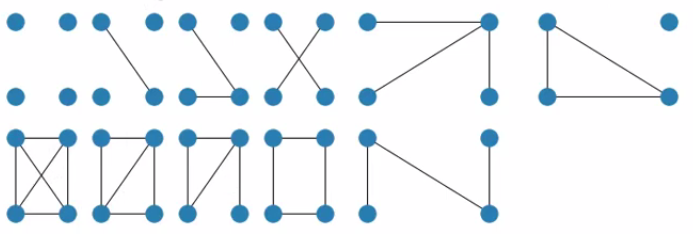
\includegraphics[scale=0.7]{img/clases-de-isomorfismo.PNG}
        \caption{Vemos que hay $11$ grafos en total}
    \end{figure}
\end{ejem}

\begin{ejem}
    Cuando escogemos dos vértices de un conjunto de vértices $X$ de tamaño $n$ no nos importa el orden, entonces el número de maneras es $n(n-1)/2 = \binom{n}{2}$. En un grafo simple, cada vértice puede formar parte de un lado o no. Al hacer esta decisión para cada par estamos especificando el grafo, entonces el número total de grafos que podemos formar a partir de $X$ es $2^{\binom{n}{2}}$.
    
    Para el ejemplo anterior vimos que hay $11$ clases de isomorfismos, pero en total tenemos $64$ grafos que podemos formar.
    
    Es notable resaltar que solamente $P_4$ es isomorfo a su complemento. Esto nos motiva a introducir la siguiente sección.
\end{ejem}

\begin{marginfigure}
    \centering
    \begin{tikzpicture}
        \GraphInit[vstyle=Normal]
        \Vertex{1}
        \Vertex[x=0 , y=3]{2}
        \Vertex[x=3 , y=3]{3}
        \Vertex[x=3 , y=0]{4}
        \tikzset{EdgeStyle/.append style = {red}}
        \Edges[color=red](1,2,4,3)
        \tikzset{EdgeStyle/.append style = {blue}}
        \Edges[color=blue](2,3,1,4)
    \end{tikzpicture}
    \caption{Vemos que $P_4 \cong P_4$}
    \label{fig:auto-complementario}
\end{marginfigure}

\subsection{Descomposición de grafos}
\stepcounter{subsec}

\begin{defn}
    Un grafo es \ul{autocomplementario} si es isomorfo a su complemento. Una \ul{descomposición} de un grafo es una lista de subgrafos tales que cada lado aparece en exactamente un subgrafo de la lista.
    
    Un grafo $H$ con $n$ vértices es autocomplementario si y sólo si $K_n$ tiene una descomposición que consiste en dos copias de $H$. El claro ejemplo de esto lo tenemos en \ref{fig:auto-complementario}.
\end{defn}

\begin{ejem}
    Otro ejemplo de un grafo autocomplementario es $C_5$. Esto lo podemos visualizar en la siguiente figura \ref{fig:auto-complementario2}.
    
    \begin{marginfigure}
        \centering
        \begin{tikzpicture}
            \SetGraphUnit{2}
            \Vertices{circle}{e,d,c,b,a}
            \tikzset{EdgeStyle/.append style = {red}}
            \Edges[color=red](a,b,c,d,e,a)
            \tikzset{EdgeStyle/.append style = {blue}}
            \Edges[color=blue](a,c,e,b,d,a)
        \end{tikzpicture}
        \caption{}
        \label{fig:auto-complementario2}
    \end{marginfigure}
\end{ejem}

Adicionalemente, tenemos las siguientes propiedades:

\begin{itemize}
    \item Todo grafo $G$ de $n$ vértices y su complemento $\overline{G}$ descomponen a $K_n$.
    \item $K_{1,n-1}$ y $K_{n-1}$ descomponen a $K_n$ a pesar de que uno de estos grafos omite un vértice.
    \item Para descomponer un grafo $H$ en copias de un grafo $G$, el número de lados de $G$ debe dividir al número de lados de $H$. Pero esto no es suficiente.
\end{itemize}

\subsection{Grafo de Petersen y automorfismos}
\stepcounter{subsec}

\begin{defn}
    El \ul{grafo de Petersen} es un grafo simple cuyos vértices son subconjuntos de $2$ elementos de un conjunto de $5$ elementos, y cuyos lados son las parejas de subconjuntos disjuntos.
    
    En otras palabras, es la clase de isomorfismo del grafo simple cuyos vértices son los pares no ordenados de elementos del conjunto $\{1,2,3,4,5\}$. Como hemos hecho con los lados de los grafos, en lugar de escribir el vértice $\{i,j\}$, escribiremos $ij$. Los lados del grafo de Petersen son todos los pares de vértices dados por conjuntos disjuntos. Por ejemplo, como $13$ y $45$ son disjuntos, los vértices $13$ y $45$ son adyacentes.
\end{defn}

\begin{figure}
    \centering
    \begin{tikzpicture}[scale=0.7]
        \SetVertexNoLabel
        \grPetersen[RA=6,RB=3]
        \AssignVertexLabel[color = blue]{a}{34,12,45,23,51}
        \AssignVertexLabel[color = blue]{b}{52,35,13,41,24}
    \end{tikzpicture}
    \caption{Grafo de Petersen}
    \label{fig:petersen}
\end{figure}

\break

\begin{nota}
    Las propiedades del grafo de Petersen se desprenden de las reglas de adyacencia que definimos anteriormente:
    
    \begin{enumerate}
        \item Cada vértice tiene grado $3$.
        \item Se descompone en dos $5$-ciclos disjuntos.
        \item Dos vértices no adyacentes tienen exactamente un vecino en común.
        \item La longitud del ciclo más corto es $5$.
    \end{enumerate}
\end{nota}

\begin{ejer}
    Para ver 3: Dos vértices no adyacentes son de la forma $ij$ e $ik$. Si $pq$ es vecino común, entonces $p$ y $q$ son ambos distintos de $i, j$ y $k$. Por lo tanto $pq$ es único, ya que queda un par par restante que podemos elegir.
    
    Para ver 4: Por $2$, basta demostrar que no tiene ciclos con menos de $5$-vértices: No tiene $1$-ciclos ni $2$-ciclos porque es un grafo simple. Un $3$-ciclo debe estar compuesto por tres vértices que corresponden a pares ordenados disjuntos, lo cual es imposible si los pares son subconjuntos de un conjunto de $5$ elementos (se necesitan al menos $6$). Supongamos ahora que el grafo contiene un $4$-ciclo. Ese ciclo no contiene $3$-ciclos, entonces tiene dos vértices no adyacentes con dos vecinos en común. Pero esto contradice 3. Entonces queda demostrado que no contiene $4$-ciclos.
\end{ejer}

\begin{defn}
    La propiedad 4 nos da pie a definir la \ul{cintura} de un grafo $G$ que tiene ciclos. Esta es la mínima longitud de un ciclo en $G$. Si un grafo no tiene ciclos se dice que su cintura es infinita.
\end{defn}

\begin{defn}
    Un \ul{automorfismo} de $G$ es un isomorfismo de $G$ a $G$. Un grafo $G$ se dice que tiene \ul{transitividad por vértices} si para cada par $u, v \in V(G)$ existe un automorfismo que envía $u$ a $v$.
\end{defn}

\begin{ejem}
    Dada una permutación $\sigma$ de $\{1,2,3,4,5\}$, la función $f_{\sigma}$ definida sobre los vértices del grafo de Petersen mediante $\Psi_{G}(ij) = \sigma(i)\sigma(j)$ preserva adyacencia. Es decir que
    
    \[
    \text{$ij$ es vecino de $pq$} \quad \iff \quad \text{$\sigma(i)\sigma(j)$ es vecino de $\sigma(p)\sigma(q)$}
    \]
    
    De esta manera, $f_{\sigma}$ es un isomorfismo del grafo de Petersen en sí mismo, un automorfismo. Esto implica que:
    
    \begin{itemize}
        \item Hay al menos $120$ automorfismos del grafo de Petersen.
        \item Para cada par de vértices en el grafo de Petersen hay un automorfismo que envía un vértice a otro, tiene transitividad por vértices.
    \end{itemize}
\end{ejem}

\begin{ejem}
    En el grafo bipartito completo $K_{n,m}$ cada permutación de una de las partes da un automorfismo, por lo tanto hay $n!m!$ en total. Si $n = m$, además de permutar los elementos de las partes, podemos permutar las partes mismas. Así que $K_{n,n}$ tiene $2(n!)^2$ automorfismos.
    
    Respecto a la transitividad por vértices, $K_{n,m}$ es transitivo por vértices sii $n = m$, ya que si $u, v$ están en distintas partes y $n \neq m$, entonces no son adyacentes a la misma cantidad de vértices, por lo tanto no se pueden permutar.
\end{ejem}

\begin{ejem}
    ¿Cuántos automorfismos tiene el camino de $4$ vértices?: Además de la identidad, la permutación $(14)(23)$\marginfootnote{Esta es la notación de ciclos, en Wikipedia aparece al buscar permutación.} es un automorfismo, ¿habrá otro? El $2$ si se mueve debe ir al $3$ (y viceversa) para preservar el grado, pero el $1$ y el $4$ no pueden quedar fijos porque se pierde la adyacencia. De esta forma, sólo hay dos automorfismos en total.
    
    Y por la discusión anterior, se concluye que para $n > 2$, $P_n$ no es transitivo por vértices.
    
    \begin{figure}
        \begin{subfigure}[b]{0.5\textwidth}
        \centering
            \begin{tikzpicture}
                \SetGraphUnit{1}
                \Vertex{1}
                \EA(1){2}
                \EA(2){3}
                \EA(3){4}
                \Edges(1,2,3,4)
            \end{tikzpicture}
            \caption{Permutación $id$.}
        \end{subfigure}
        \hfill
        \begin{subfigure}[b]{0.5\textwidth}
        \centering
            \begin{tikzpicture}
                \SetGraphUnit{1}
                \Vertex{4}
                \EA(4){3}
                \EA(3){2}
                \EA(2){1}
                \Edges(1,2,3,4)
            \end{tikzpicture}
            \caption{Permutación $(14)(23)$.}
        \end{subfigure}
    \end{figure}
\end{ejem}
\section{Paseos, recorridos y ciclos}
\stepcounter{sec}

En la parte anterior definimos los caminos, pero dependiendo del problema, querremos modelarlo prestando atención en el movimiento dentro del grafo. Quizá nos interese fijarnos en los vértices recorridos o en los lados recorridos.

\subsection{Conexidad}
\stepcounter{subsec}

\begin{defn}
    Un \ul{paseo} $W$ es una lista $v_0, e_1, v_2, \dots, e_k, v_k$ de vértices y lados de un grafo $G$ tales que para $i = 1, \dots, k$ se tiene $f_G(e_k) = \{v_{j-1},v_j\}$. Vemos que $k$ es la cantidad de lados del paseo, y lo denotaremos por $k = \lngtd{W}$.
    
    Un \ul{recorrido} es un paseo sin lados repetidos, es decir que si $W$ es un paseo en $G$, entonces $\forall i,j$ tenemos que $i \neq j \implies e_i \neq e_j$, con $e_i, e_j \in W$.
    
    Diremos que un paseo es \ul{cerrado} si $v_0 = v_k$.
\end{defn}

Es inmediato suponer que existe una relación entre los paseos y los caminos (que definimos en la sección anterior). Veamos concretamente cómo se relacionan:

\begin{lem}
    Todo paseo de $u$ a $v$ contiene un camino de $u$ a $v$.
\end{lem}

\begin{proof}
    Pasaremos a realizar la demostración de este lema por inducción: Sea $W$ un camino con $\lngtd{W} = n$. Si $n = 0$, entonces el paseo no tiene lados, por lo tanto $W$ consiste de un único vértice y $u = v$. De esta forma $W$ contiene un camino de $u$ a $v$ de longitud $0$.
    
    \begin{marginfigure}
        \centering
        \begin{tikzpicture}
            \SetGraphUnit{1}
            \Vertex{u}
            \WE(u){v1}
            \WE(v1){v2}
            \WE(v2){v3}
            \WE(v3){w}
            \SO(w){v}
            \Edges(u,v1,v2,v3,w,v)
            \Loop[dist=1cm](w)
        \end{tikzpicture}
        \caption{Situación descrita en la demostración del lema. El bucle en $w$ representa los vértices entre $w$ y su repetición. Al igual que ocurre en $w$, esta situación se puede generalizar para cualquier vértice.}
    \end{marginfigure}
    
    Supongamos ahora que el teorema se cumple para $n < k$. Toca demostrar para $n = k$: Si $W$ no tiene vértices repetidos, entonces todos sus vértices y lados forman un camino de $u$ a $v$. Si $W$ tiene un vértice repetido $w$, entonces omitamos todos los lados y vértices que aparecen entre $w$ y su repetición, de esta forma obtenemos un paseo $W'$ contenido en $W$. Como $\lngtd{W'} < k$, podemos aplicar la H.I y hay un camino $P$ de $u$ a $V$ contenido en $W'$. Ya que $W' \subset W$, entonces el camino $P$ está contenido en $W$.
    
    De esta forma, hemos demostrado el lema por inducción.
\end{proof}

\begin{defn}
    Sean $G$ un grafo y $u, v \in G$. Diremos que $x$ está \ul{conectado} con $y$ si existe un camino de $u$ a $v$ (y de lo contrario, \ul{desconectado}). La \ul{relación de conexidad} sobre $V(G)$ consiste en los pares ordenados $(u,v)$ tales que $u$ está conectado a $v$. Las clases de equivalencia de esta relación son las componentes del grafo $G$, es decir todo subgrafo de $G$ tal que es conexo maximal.
\end{defn}

\begin{ejem}\label{ejem:cortes}
    El grafo de abajo tiene $4$ componentes, una de ellas siendo un vértice aislado. Los conjuntos de vértices de cada componente son $\{a,b\}$, $\{c,d,e,f,g\}$, $\{h\}$ e $\{i,j,k\}$, y estas son las clases de equivalencia respecto a la relación de conexidad.
    
    \begin{figure}
        \centering
        \begin{tikzpicture}
            \SetGraphUnit{1}
            \Vertex{a}
            \SO(a){b}
            \Edges(a,b)
            \Vertex[x=1 , y=0]{c}
            \EA(c){d}
            \SO(d){g}
            \EA(d){e}
            \EA(e){f}
            \Edges(c,g,d,c,d,e,g,e,f)
            \Vertex[x=3.5 , y=-1]{h}
            \Vertex[x=5 , y=-1]{i}
            \Vertex[x=5.5 , y=0]{j}
            \EA(j){k}
            \Edges(i,j,k)
        \end{tikzpicture}
        \caption{Grafo con $4$ componentes.}
    \end{figure}
\end{ejem}

Vemos del ejemplo anterior que eliminar un vértice o lado puede incrementar el número de componentes. Por ejemplo, si eliminamos el lado que incide en $i$ pasamos a tener $5$ componentes, lo mismo ocurre si eliminamos $j$ y los lados que inciden con él.

\begin{defn}
    Un \ul{lado-corte} ó \ul{vértice-corte} de un grafo es un lado o vértice que al retirarlo del grafo incrementa el número de componentes. Escribimos $G - e$ o $G - M$ para denotar al subgrafo de $G$ obtenido al retirar el lado $e$ o el conjunto de lados $M$. Escribimos $G - v$ ó $G - S$ para denotar al subgrafo obtenido al retirar el vértice $e$ o el conjunto de vértices $S$.
\end{defn}

Es importante resaltar que las componentes son disjuntas dos a dos, es decir que no existe un par de componentes que comparta un vértice. Añadir un lado que une a dos vértices en componentes distintas hace que se reduzca en $1$ el número de componentes. De esta forma, añadir un lado reduce el número de componentes en $0$ o en $1$, y eliminar un lado incrementa el número de componentes por $0$ o $1$.

\begin{pro}
    Todo grafo con $n$ vértices y $k$ lados tiene al menos $n-k$ componentes.
\end{pro}

\begin{proof}
    Un grafo con $n$ vértices sin lados tiene $n$ componentes. Sabemos por la discusión anterior que cada lado reduce el número en componentes en máximo $1$, así que cuando se han añadido $k$ lados, el número de componentes sigue siendo mayor o igual a $n-k$.
\end{proof}

\begin{ejem}
    Para el grafo presentado en el ejemplo \ref{ejem:cortes}, tenemos que
    
    \begin{itemize}
        \item Lados-corte: $ab$, $ef$, $ij$, $jk$.
        \item Vértices-corte: $e$, $j$.
    \end{itemize}
\end{ejem}

\begin{defn}
    Sean $G$ un grafo y $T \subseteq V(G)$. El \ul{grafo inducido} denotado por $G[T]$ está conformado por $T$, $f_G$ y todo lado $e \in E(G)$ que cumpla lo siguiente: para algún par no ordenado $\{u,v\}$ con $u,v \in V(T)$, se tiene que $\{u,v\} = f_G(e)$. Es decir, que el grafo inducido consiste también de todos los lados cuyos vértices están contenidos en $V(T)$.
\end{defn}

Para esta definición, es importante resaltar que un conjunto de vértices $S$ es un conjunto independiente sii el grafo inducido por $S$ no tiene lados.

\begin{ejem}
    Nuevamente, en el grafo del ejemplo \ref{ejem:cortes}, tenemos que $C_4$ y $P_5$ son subgrafos \textbf{NO} inducidos, y $P_4$ es un subgrafo inducido: Puede ser inducido por $\{c,g,e,f\}$ o por $\{c,d,e,f\}$.
\end{ejem}

\begin{teo}
    Sean $G$ un grafo y $e \in E(G)$, entonces $e$ es un lado-corte sii no pertenece a un ciclo.
\end{teo}

\begin{proof}
    Sea $e$ un lado de un grafo $G$ (con vértices $x,y$) y sea $H$ la componente que contiene a $e$. Como al eliminar $e$ ninguna otra componente se ve afectada, es suficiente probar que $H - e$ es conexo si y sólo si $e$ pertenece a un ciclo. Probemos ambas implicaciones:
    
    \begin{enumerate}
        \item[$\Leftarrow$] Supongamos que $e$ pertenece a un ciclo $C$ de $H$. Escojamos $u, v \in V(H)$. Como $H$ es conexo, entonces $H$ tiene un camino $P$ de $u$ a $v$. Si $P$ no contiene a $e$, entonces $P$ está en $H - e$, como esto es para todo $u, v \in V(H)$, $H - e$ es conexo. Si $P$ contiene a $e$ supongamos en primer lugar y sin pérdida de generalidad que $x$ está entre $u$ e $y$ en $P$. Como $H - e$ contiene un camino de $u$ a $x$ (el cual está en $P$), un camino de $x$ a $y$ (está en $C$) y un camino de $y$ a $v$ (está en $P$ nuevamente), por la transitividad de la relación de conexidad tenemos que eso implica que $H - e$ tiene un camino de $u$ a $v$, y esto se cumple para todo $u, v \in V(G)$.
        
        De esta forma, $u, v \in V(H)$ y $H - e$ es conexo.
        
        \item[$\Rightarrow$] Supongamos ahora que $H - e$ es conexo. Esto implica que existe un camino de $x$ a $y$, y si se agrega nuevamente el lado $e$, se tiene un ciclo. Por lo tanto $e$ pertenece a un ciclo.
    \end{enumerate}
    
    De esta manera queda demostrado.
\end{proof}
\section{Grafos y conteo}
\stepcounter{sec}

Algunas de las preguntas que ahora son relevantes y que contestaremos en esta sección son las siguientes:

\begin{itemize}
    \item ¿Cómo se relaciona la cantidad de lados de un grafo con la cantidad de vértices?
    \item ¿Cuántos subgrafos con características dadas, tiene un grafo?
    \item ¿Cuántas clases de isomorfismo tiene un grafo dado?
\end{itemize}

\begin{defn}
    Antes de hacer los análisis pertinentes, vale la pena recordar algunos conceptos y notación e introduciremos algunos más:
    
    \begin{enumerate}
        \item El \ul{grado} de $v \in V(G)$ es la cantidad de lados de $G$ incidentes con $v$ (si $v$ tiene bucles, estos contribuyen en $2$ al grado). Lo denotaremos por $d_G(v)$ ó $d(v)$.
        \item $\Delta(G)$ es el máximo de los grados en $G$.
        \item $\delta(G)$ es el mínimo de los grados en $G$.
        \item Si $\Delta(G) = \delta(G) = k$, decimos que $G$ es \ul{$k$-regular}.
        \item La \ul{vecindad} de $v \in V(G)$ es el conjunto $N_G(v)$ de los vecinos de $v$ en $G$.
        \item El \ul{orden} de $G$ es $n(G) = |V(G)|$.
        \item El \ul{tamaño} de $G$ es $e(G) = |E(G)|$.
        \item Dado $n \in \N$, denotamos $[n] = \{1, 2, \dots, n\}$.
    \end{enumerate}
\end{defn}

\subsection{Conteo y biyecciones}
\stepcounter{subsec}

Introduciremos esta subsección con un resultado bastante relevante: Si queremos calcular la suma de los grados de los vértices de $G$, cada lado se cuenta dos veces. Hemos demostrado el siguiente resultado:

\begin{teo}[Primer Teorema de la Teoría de Grafos]\label{teo:primer}
    Si $G$ es un grafo, entonces
    
    \[
    \sum_{v \in V(G)} d(v) = 2e(G)
    \]
\end{teo}

De este teorema se pueden sacar varios corolarios:

\begin{cor}
    En un grafo $G$, el promedio de los grados es
    
    \[
    \frac{2e(G)}{n(G)}
    \]
    
    Por lo tanto,
    
    \[
    \delta(G) \leq \frac{2e(G)}{n(G)} \leq \Delta(G)
    \]
\end{cor}

\begin{cor}
    $G$ tiene una cantidad par de vértices con grado impar.
\end{cor}

\begin{cor}
    Si $G$ es $k$-regular, entonces $e(G) = kn(G)/2$.
\end{cor}

\begin{cor}
    Si $n(G)$ es impar y $G$ es $k$-regular, entonces $k$ no puede ser impar.
\end{cor}

\begin{defn}
    El \ul{cubo $k$-dimensional} o \ul{hipercubo} $Q_k$, es el grafo simple cuyos vértices son las $k$-tuplas con entradas en $\{0,1\}$ y cuyos lados son las parejas de $k$-tuplas que difieren en \textbf{exactamente} una posición.
\end{defn}

\begin{figure}
    \centering
    \begin{tikzpicture}
        \SetGraphUnit{2}
        \SetVertexNoLabel
        \grCycle[rotation=45, prefix=a, RA=1]{4}
        \grCycle[x=3, y=1.5, rotation=45, prefix=b, RA=1]{4}
        \AssignVertexLabel{a}{000,100,110,010}
        \AssignVertexLabel{b}{001,101,111,011}
        \SetUpEdge[style={dashed}]
        \Edge(a0)(b0)
        \Edge(a1)(b1)
        \Edge(a2)(b2)
        \Edge(a3)(b3)
    \end{tikzpicture}
    \caption{Acá se puede apreciar una representación de $Q_3$}
    \label{fig:hipercubo}
\end{figure}

\begin{prob}[Estructura de los hipercubos]
    Con respecto a los hipercubos surjen muchísimas propiedades interesantes:
    
    \begin{itemize}
        \item Podemos establecer la \textit{paridad} de un vértice de $Q_k$ la siguiente manera: Si tiene una cantidad par de $1$s es par, y de lo contrario es impar. Cada lado de $Q_k$ incide en un vértice par y otro impar. De esta forma, los vértices pares son adyacentes únicamente a los impares, y viceversa. Por lo tanto ambos conjuntos de vértices forman un conjunto independiente y tenemos como resultado que $Q_k$ es bipartito.
        \item Cada posición en las $k$-tuplas se puede elegir de dos maneras, por lo tanto $n(Q_k) = 2^k$. Además, los vecinos de cada vértice se pueden obtener al cambiar una de las $k$ posiciones de la tupla, por lo tanto $Q_k$ es $k$-regular, y se tiene que $e(Q_k) = k2^{k-1}$.
        \item Vemos en la figura \ref{fig:hipercubo} que los lados no punteados son dos subgrafos de $Q_3$ isomorfos a $Q_2$, formados al mantener fijas la última coordenada de las tuplas. ¿De qué manera podemos generalizar este resultado?: Podemos formar un subcubo $j$-dimensional al fijar $k-j$ coordenadas y hacer que los valores en las $j$ sean escogidos a partir de una de las $2^j$ $j$-tuplas restantes. El subgrafo inducido por este conjunto de vértices es isomorfo a $Q_j$. Como hay $\binom{k}{j}$ maneras para escoger las $j$ coordenadas a variar, y $2^{k-j}$ maneras de escojer las coordenadas fijas y sus valores, en total tenemos $\binom{k}{j}2^{k-j}$ subcubos. Así, para cada $j \leq k$, $Q_k$ tiene $\binom{k}{j}2^{k-j}$ subgrafos isomorfos a $Q_j$.
    \end{itemize}
    
    % Maldita sea como me excitan los hipercubos
    Ahora, ¿cómo podemos construir un hipercubo $Q_k$?: Agregar $0$ a las tuplas de una copia de $Q_{k-1}$, agregar $1$ a las tuplas de otra copia de $Q_{k-1}$, y unir los vértices cuyas primeras $k-1$ coordenadas sean iguales. El resultado será $Q_k$.
\end{prob}

Vimos que un hipercubo es un grafo regular y bipartito, a continuación estableceremos una observación fundamental sobre esos grafos.

\begin{teo}
    Si $k > 0$, entonces un grafo $k$-regular y bipartito tiene la misma cantidad de vértices en cada partición.
\end{teo}

\begin{proof}
    Sea $G$ un grafo $k$-regular y bipartito. Supongamos que $\{A, B\}$ es la bipartición. Entonces cada lado de $G$ tiene un extremo en $A$, por lo tanto $e(G) = k|A|$. También cada lado de $G$ tiene un extremo en $B$, por lo tanto $e(G) = k|B|$. Esto implica que $|A| = |B|$.
\end{proof}

\break

Otra técnica de conteo para conjuntos involucra establecer una biyección desde el conjunto a otro de un tamaño conocido. El siguiente problema utiliza este enfoque.

\begin{prob}
    ¿Cuántos $6$-ciclos tiene el grafo de Petersen?
\end{prob}


\section{Grafos dirigidos}
\stepcounter{sec}

Hasta ahora hemos utilizado los grafos para modelar relaciones simétricas, pero en general este no tiene por qué ser el caso. Por ejemplo, en algunas redes se puede \textit{seguir} a alguien y éste no necesariamente te sigue. En estos casos decimos que la relación va en una \textit{dirección}. Esto se refleja gráficamente partiendo de la idea de un grafo: Solo hace galta agregar la dirección en los lados, lo que indica el orden de la relación.

\begin{defn}
    Un \ul{digrafo} o \ul{grafo dirigido}, es una tripleta $G = ( V(G), E(G), f_G)$ en el cual $V(G)$ y $E(G)$ son conjuntos (de vértices y lados) y $f_G: E(G) \rightarrow V(G) \times V(G)$.
    
    Si $(v,w) = f_G(e)$ para algún $e \in E(G)$, entonces decimos que $v$ es la \ul{cola} de $e$, y $w$ es la \ul{cabeza} de $e$. En este caso, escribimos $v \rightarrow w$ y también decimos que $v$ es \ul{predecesor} de $w$, y $w$ es \ul{sucesor} de $v$.
    
    Los lados cuyas imágenes tienen la forma $(v,v)$ son \ul{bucles} y si $f_G$ no es inyectiva, decimos que $G$ tiene lados \ul{múltiples}. Si $f_G$ es inyectiva, entonces decimos que $G$ es simple. Se observa que un digrafo simple $G$ puede tener bucles. Como antes, denotaremos $|V(G)| = n(G)$, $|E(G)| = e(G)$.
\end{defn}

\begin{ejem}
    \begin{marginfigure}
        % Falta hacer el digrafo
        \centering
        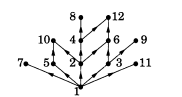
\includegraphics{img/digrafo.PNG}
        \caption{Ejemplo de digrafo.}
        \label{fig:digrafo}
    \end{marginfigure}
    
    Vemos en la figura \ref{fig:digrafo}~que $V(G) = [12]$, $E(G)$ está formado por las flechas y $f_G(e) = (t,h)$ si $h/t$ es primo. En este caso, el digrafo es simple.
\end{ejem}

\begin{ejem}
    \begin{marginfigure}
        % Falta hacer el digrafo
        \centering
        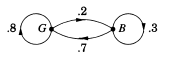
\includegraphics{img/markov.PNG}
        \caption{Cadena de Markov.}
        \label{fig:markov}
    \end{marginfigure}
    
    Los digrafos son útiles para modelar sistemas en los que los vértices representan estados, y los lados representan transición entre ellos. Un sistema cuyos estados cambian de forma aleatoria se llama \textbf{cadena de Markov}. Por ejemplo, en la figura \ref{fig:markov}~tenemos representados a los estados del tiempo con $G$ (bueno) y $B$ (malo). Las probabilidades son:
    
    \begin{enumerate}
        \item Que un día bueno siga siendo bueno: $0.8$.
        \item Que un día bueno se haga malo: $0.2$.
        \item Que un día malo siga siendo malo: $0.3$.
        \item Que un día malo se haga bueno: $0.7$.
    \end{enumerate}
\end{ejem}

\begin{defn}
    Dado un digrafo $D$, el \ul{grafo base} $G$ de $D$ se obtiene con los vértices de $D$ y considerando los lados sin tomar en cuenta el orden de los pares.
\end{defn}

\begin{defn}
    Un digrafo simple es un \ul{camino} si sus vértices se pueden ordenar de la forma $v_1, v_2, \dots, v_n$ con $v_i \rightarrow v_j$ si y sólo si $j = i+1$. En este caso decimos que se trata de un camino de $v_1$ a $v_n$.
    
    Un digrafo simple es un \ul{ciclo} si sus vértices se pueden ordenar de la forma $v_1, \dots, v_n$ con $v_i \rightarrow v_j$ si y sólo si $j = i+1$ ó $i=n$ y $j=1$.
    
    Otros conceptos visto para grafos son análogos para grafos:
    
    \begin{itemize}
        \item Subdigrafo.
        \item Isomorfismo (digrafos isomorfos, clases de isomorfismo).
        \item Descomposición de digrafos.
        \item Unión de digrafos.
    \end{itemize}
\end{defn}

Otros conceptos requieren modificaciones, o tienen algunas diferencias:

\begin{defn}
    Dado un digrafo $G$:
    
    \begin{itemize}
        \item Una \ul{matriz de incidencia} (si $G$ no tiene bucles) $M(G)$ está dada por $m_{ij} = 1$ si $x_i$ es la cola de $e_j$ y $m_{ij} = -1$ si $v_i$ es la cabeza de $e_j$.
        \item Una \ul{matriz de adyacencia} $A(G)$ está dada por $a_{ij} =$~cantidad de lados correspondientes a $v_i \rightarrow v_j$.
    \end{itemize}
    
    \begin{figure}
        \centering
        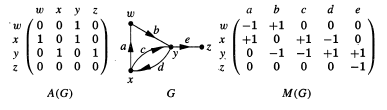
\includegraphics{img/matrices.PNG}
        \caption{}
        \label{fig:matrices}
    \end{figure}
\end{defn}

\begin{defn}
    Dados dos vértices $v,w$ de un digrafo, es posible que existe un camino de $v$ a $w$ y que no exista un camino de $w$ a $v$. Dado un digrafo $G$ con grafo base $G$, decimos que
    
    \begin{enumerate}
        \item $D$ es \ul{débilmente conexo} si $G$ es conexo.
        \item $D$ es \ul{conexo (o fuertemente conexo)} si para cada par ordenado de vértices $v,w$, existe un camino de $v$ a $w$ en $D$.
    \end{enumerate}
\end{defn}

\subsection{Grados y suceciones gráficas}
\stepcounter{subsec}

\begin{defn}
    Dados un digrafo $G$ y $v \in V(G)$,
    
    \begin{itemize}
        \item El \ul{grado de entrada} de $v$ en $G$ es la cantidad $d_G^-(v)$ de lados que tienen a $v$ como cabeza.
        \item El \ul{grado de salida} de $v$ en $G$ es la cantidad $d_G^+(v)$ de lados que tienen a $v$ como cola.
        \item El conjunto de \ul{predecesores} de $v$ es $N_G^-(v) \{w \in V(G) : w \rightarrow v\}$.
        \item El conjunto de \ul{sucesores} de $v$ es $N_G^+(v) \{w \in V(G) : v \rightarrow w\}$.
        \item $\delta^-(G) = \min \{d_G^-(w) : w \in V(G)\}$.
        \item $\Delta^-(G) = \max \{d_G^-(w) : w \in V(G)\}$.
        \item $\delta^+(G) = \min \{d_G^+(w) : w \in V(G)\}$.
        \item $\Delta^-(G) = \max \{d_G^+(w) : w \in V(G)\}$.
    \end{itemize}
\end{defn}

\begin{teo}
    En un digrafo $G$, tenemos que
    
    \[
    \sum_{v \in V(G)} d^+(v) = e(G) = \sum_{v \in V(G)} d^-(v)
    \]
\end{teo}

\begin{proof}
    Cada lado tiene exactamente una sola cola y una sola cabeza.
\end{proof}

Ahora, si quisiéramos definir sucesiciones (di)gráficas, tendrían que ser sucesiones de pares de números $(d_1^+,d_1^-), \dots, (d_n^+,d_n^-)$.

\begin{teo}
    Una lista de pares ordenados de enteros no negativos es realizable por un digrafo sii la suma de las primeras coordenadas es igual a la suma de las segundas coordenadas.
\end{teo}

\begin{proof}
    La condición es necesaria porque todo lado tiene una cola y una cabeza, contribuyendo cada uno exactamente uno a cada suma.
    
    Para ver la suficiencia, consideremos las parejas
    
    \[
    \{ (d_i^+, d_i^-) : 1 \leq i \leq n \}
    \]
    
    \noindent y los vértices $v_1, \dots, v_n$. Sea ahora $\sum_{j=1}^n d_j^- = \sum_{i=1}^n d_i^+ = m$. Consideremos los $n$ vértices y construyamos $m$ pares ordenados de la siguiente manera:
    
    Para cada $i$, se coloca $i$ en las primeras $d_i^+$ coordenadas. Para cada $j$, se coloca $-j$ en las primeras $d_j^-$ coordenadas. Para cada $(i,-j)$ agregamos un lado de $v_i$ a $v_j$. El digrafo resultante realiza $(d_1^+, d_1^-), \dots, (d_n^+, d_n^-)$.
    
    Así, queda demostrado el teorema.
\end{proof}

Para este teorema permitimos lados múltiples, ¿cómo podemos estudiar una versión análoga para digrafos simples?. Nos valdremos de una técnica que hace uso de los grafos bipartitos:

\begin{defn}
    El \ul{split} de un digrafo $D$ es un grafo bipartito $G$ cuyos conjuntos bipartitos $V^+$, $V^-$ son copias de $V(D)$. Para cada vértice $x \in V(D)$, tenemos un vértice $x^+ \in V^+$ y un vértice $V^- \in V^-$. Para cada lado $u,v \in E(D)$, hay un lados con extremos $u^+, v^- \in G$.
\end{defn}

\begin{figure}
    \centering
    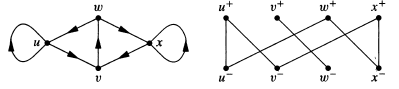
\includegraphics{img/split.PNG}
    \caption{Ejemplo de split.}
    \label{fig:split}
\end{figure}

En la figura \ref{fig:split}~se observa que los grados en $G$ corresponden a los grados de salida y entrada en $D$.

Más aún, dado un grafo bipartito $G$ con bipartición $X$, $Y$ tal que $|X| = |Y| = n$, se puede revertir el proceso para obtener un digrafo $D$ tal que $G$ sea su split. Aquí se ve claro por qué permitimos bucles en los digrafos simples.

Entonces, dada $(d_1^+,d_1^-), \dots, (d_n^+,d_n^-)$ tal que la suma de las primeras coordenadas es igual a la suma de las segundas, existe un digrafo simple que la realiza si y sólo si existe un grafo $G$, bipartito con particiones $X$ e $Y$ tal que $|X| = |Y| = n$, donde los $d_j^+$ son grados en $X$ y los $d_j^-$ son los grados en $Y$.

\subsection{El digrafo de De Bruijin}
\stepcounter{subsec}

Es sencillo dar los conceptos de \textit{paseo} y \textit{recorrido} para digrafos. A partir de allí se puede definir de inmediato \textit{recorridos eulerianos}, \textit{circuitos eulerianos} y \textit{digrafos eulerianos}. De hecho, para obtener una caracterización de los digrafos eulerianos en función de los grados de los vértices, basta con un par de resultados sencillos.

\begin{lem}
    Si $G$ es un digrafo tal que $\delta^+(G) \geq 1$ ó $\delta^-(G) \geq 1$, entonces $G$ tiene un ciclo.
\end{lem}

\begin{proof}
    Supongamos que $G$ es un digrafo para el cual $\delta^+(G) \geq 1$. Sea $P$ un camino maximal en $G$. Si $u$ es el último vértice de $P$, $u$ tiene un sucesor en $P$. De esta manera, obtenemos un ciclo en $G$. Para demostrar cuando $\delta^-(G) \geq 1$, el razonamiento es totalmente análogo.
\end{proof}

\begin{teo}
    Un digrafo $G$ es euleriano sii para cada $v \in V(G)$ vale $d^+(G) = d^-(G)$ y el grado base de $G$ a lo sumo tiene una componente no trivial.
\end{teo}

\begin{proof}
    Queda como ejercicio. Se demuestra usando inducción y el lema anterior.
\end{proof}

Ahora, pasemos a observar la siguiente sucesión binaria:

\[
0000111101100101
\]

Esta cumple con lo siguiente:

\begin{enumerate}
    \item Cada bloque de $4$ dígitos consecutivos es distinto.
    \item Si esto se ve de forma cíclica, es aparente que están todos los $4$-bloques posibles.
\end{enumerate}

Esto es un ejemplo de lo que se conoce como \textbf{ciclo de De Bruijin}. En general, un ciclo de De Bruijin es una cadena de longitud $2^n$ tal que, vista de forma cíclica, contiene todos los $n$-bloques binarios distintos. Dado $n$, ¿existe un ciclo de De Bruijin para ese $n$? Si es así, ¿cómo se puede construir?

Volvamos al ejemplo que dimos anteriormente ($n=4$). Usaremos un digrafo $D_4$ construído de la siguiente manera:

\begin{enumerate}
    \item Los vértices de $D_4$ son cadenas binarias de $3$ dígitos.
    \item $u \rightarrow v$ si los últimos $2$ dígitos de $u$ coinciden con los primeros de $v$.
    \item Etiquetamos el lado $u \rightarrow v$ con el último dígito de $v$.
    \item $D_4$ es euleriano.
    \item Las etiquetas de los lados de cualquier circuito euleriano en $D_4$ forman un ciclo de De Bruijin.
\end{enumerate}

\begin{figure}
    \centering
    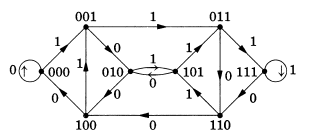
\includegraphics{img/de-bruijin.PNG}
    \caption{Ciclo de De Bruijin $D_4$.}
    \label{fig:de-bruijin}
\end{figure}

Vemos que en general, dado $n$ tenemos que los vértices de $D_n$ son las cadenas binarias con $n-1$ dígitos, si $u \rightarrow v$ los últimos $n-2$ dígitos coinciden con los primeros $n-2$ de $v$, y se etiqueta al lado $u \rightarrow v$ con el último dígito de $v$.

Esto nos motiva a el siguiente teorema:

\begin{teo}
    Para cada $n$, $D_n$ es euleriano y las etiquetas de cada ciclo euleriano en $D_n$ definen un diclo de De Bruijin.
\end{teo}

\begin{proof}
    Sea $D_n$. Entonces al agregar $0$ o $1$ al final de un vértice y eliminar el primero, obtenemos un sucesor, por lo que $d^+(v) = 2$ para todo $v \in V(D_n)$, y cada vértice es sucesor de otro que comienza en $1$ y otro que comienza en $0$, por lo tanto $d^-(v) = 2$. Entonces $d^+(v) = d^-(v) = 2$ para cada $v$. Más aún, dado un vértice $b_1b_2 \dots b_{n-1}$ podemos llegar a él desde cualquier otro vértice, siguiente los lados etiquetados con $b_1, b_2, \dots$. Por lo tanto $D_n$ es euleriano.
    
    Ahora, para llegar a un vértice $v = b_1b_2 \dots b_{n-1}$, debe haber sido a través de lados con etiquetas $b_1, \dots, b_{n-1}$. Si desde $v$ se usa un lado etiquetado con $b_n$, se obtiene la cadena $b_1b_2 \dots b_n$. Como los vértices son cadenas distintas, tenemos todas las cadenas binarias (distintas) de longitud $n$ usando un ciclo euleriano.
\end{proof}

\subsection{Orientaciones y torneos}
\stepcounter{subsec}

Para introducir el concepto de torneos, presentamos el siguiente problema:

\begin{prob}
    En varios deposrtes se hacen torneos tipo \textit{round robin}: cada equipo se enfrenta a otro sólo una vez y no hay empates. Si son $n$ equipos, ¿cuántos resultados son posibles en un torneo así?
    
    Podemos modelar el resultado con un digrafo:
    
    \begin{itemize}
        \item Cada equipo es un vértice.
        \item Todos los vértices son vecinos dos a dos.
        \item Si $x$ derrota a $y$ entonces escribimos $x \rightarrow y$.
        \item En cada juego hay dos posibilidades $x \rightarrow y$ ó $y \rightarrow x$.
    \end{itemize}
    
    \begin{marginfigure}
        \centering
        \begin{tikzpicture}
            \GraphInit[vstyle=Classic]
            \SetVertexNoLabel
            \grComplete[RA=2]{6}
            \tikzset{EdgeStyle/.append style = {red}}
            \Edge[style={->}, color=red](a0)(a1)
            \Edge[style={->}, color=red](a0)(a2)
            \Edge[style={->}, color=red](a0)(a4)
            \Edge[style={->}, color=red](a5)(a0)
            \Edge[style={->}, color=red](a3)(a0)
            \Edge[style={->}, color=red](a2)(a1)
            \Edge[style={->}, color=red](a1)(a3)
            \Edge[style={->}, color=red](a1)(a4)
            \Edge[style={->}, color=red](a5)(a1)
            \Edge[style={->}, color=red](a3)(a2)
            \Edge[style={->}, color=red](a2)(a4)
            \Edge[style={->}, color=red](a5)(a2)
            \Edge[style={->}, color=red](a4)(a5)
            \Edge[style={->}, color=red](a5)(a3)
            \Edge[style={->}, color=red](a3)(a4)
        \end{tikzpicture}
        \caption{Torneo de 6 vértices.}
        \label{fig:torneo}
    \end{marginfigure}
    
    Observémos las características del digrafo \ref{fig:torneo}~, no hay lados múltiples, no hay bucles y cada vértice es vecino de todos los demás.
\end{prob}

Todo esto nos permite establecer las siguientes definiciones:

\begin{defn}
    Una \ul{orientación} de un grafo $G$ es un digrafo $D$ obtenido a partir de $G$ al escoger una orientación $x \rightarrow y$ ó $y \rightarrow x$ para cada lado $xy \in E(G)$. Un \ul{grafo orientado} es una orientación de un grafo simple sin bucles. Un \ul{torneo} es una orientación de un grafo completo.
\end{defn}

\begin{prob}
    ¿En general, cuántos digrafos con $n$ vértices hay?: En primer lugar, hay $n^2$ pares ordenados de vértices (permitiendo bucles). Un digrafo simple permite bucles pero usa cada par ordenado a lo sumo una vez como lado, por lo tanto existen $2^{n^2}$ conjuntos de lados posibles.
    
    Por otro lado, modifiquemos el análisis para las orientaciones de un grafo simple con $n$ vértices: Hay $\binom{n}{2}$ pares no ordenados de vértices, y para cada par no ordenado de vértices $\{x,y\}$ hay tres posibilidades, son no adyacentes, $x \rightarrow y$ ó $y \rightarrow x$. Entonces hay en total $3^{\binom{n}{2}}$ orientaciones. Para torneos, sólo hay dos posibilidades, $x \rightarrow y$ ó $y \rightarrow x$. Por lo tanto hay $2^{\binom{n}{2}}$ torneos con $n$ vértices.
\end{prob}

En un torneo con $n$ vérticces es muy probable que más de un equipo tenga grado de salida máximo. ¿Cómo decidimos el campeón de un torneo? Una posibilidad es buscar un equipo $x$ con la propiedad:

\begin{enumerate}
    \item Dado un equipo $x$, $x$ derrota a $z$ o $x$ derrota a algún $y$ que derrota a $z$.
\end{enumerate}

Más formalmente, definimos:

\begin{defn}
    En un digrafo, un \ul{rey} es un vértice desde el cual cualquier otro vértice puede ser alcanzado mediante un camino de longitud a lo sumo $2$.
\end{defn}

Ahora, vale la pena preguntarse: Dado un torneo $T$, ¿existe un rey en $T$?

\begin{teo}[Landau, 1953]
    Todo torneo infinito tiene un rey.
\end{teo}

\begin{proof}
    Sea $x$ un vértice en un torneo $T$. Si $x$ no es un rey, entonces algún vértice $y$ no puede alcanzarse desde $x$ con un camino de a lo sumo longitud $2$. Por lo tanto ningún sucesor de $x$ es un predecesor de $y$. Como $T$ es una orientación de un clique, todo sucesor de $x$ debe ser sucesor de $y$, y además $y \rightarrow x$. Por lo tanto $d^+(y) > d^+(x)$.
    
    Si $y$ no es un rey, entonces repetimos el argumento para encontrar $z$ con un grado de salida más grande. Como $T$ es finito, este procedimiento termina. Y este termina solamente si hemos encontrado un rey.
\end{proof}

\end{document}